% This file was created by matlab2tikz.
%
\documentclass[tikz]{standalone}
\usepackage[T1]{fontenc}
\usepackage[utf8]{inputenc}
\usepackage{pgfplots}
\usepackage{grffile}
\pgfplotsset{compat=newest}
\usetikzlibrary{plotmarks}
\usetikzlibrary{arrows.meta}
\usepgfplotslibrary{patchplots}
\usepackage{amsmath}

\newlength\figureHeight \setlength{\figureHeight}{6cm}
\newlength\figureWidth \setlength{\figureWidth}{10cm}
\begin{document}
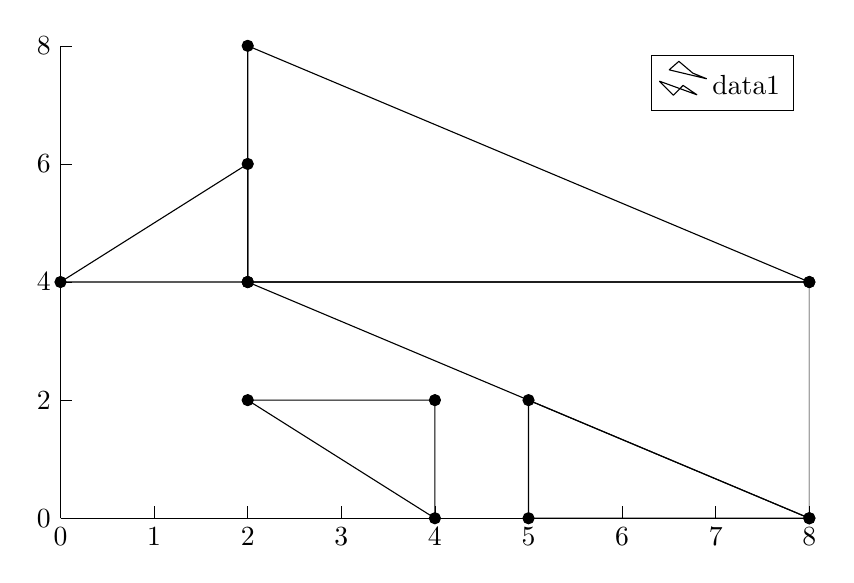
\begin{tikzpicture}

\begin{axis}[%
width=0.951\figureWidth,
height=\figureHeight,
at={(0\figureWidth,0\figureHeight)},
scale only axis,
colormap={mymap}{[1pt] rgb(0pt)=(0.2422,0.1504,0.6603); rgb(1pt)=(0.25039,0.164995,0.707614); rgb(2pt)=(0.257771,0.181781,0.751138); rgb(3pt)=(0.264729,0.197757,0.795214); rgb(4pt)=(0.270648,0.214676,0.836371); rgb(5pt)=(0.275114,0.234238,0.870986); rgb(6pt)=(0.2783,0.255871,0.899071); rgb(7pt)=(0.280333,0.278233,0.9221); rgb(8pt)=(0.281338,0.300595,0.941376); rgb(9pt)=(0.281014,0.322757,0.957886); rgb(10pt)=(0.279467,0.344671,0.971676); rgb(11pt)=(0.275971,0.366681,0.982905); rgb(12pt)=(0.269914,0.3892,0.9906); rgb(13pt)=(0.260243,0.412329,0.995157); rgb(14pt)=(0.244033,0.435833,0.998833); rgb(15pt)=(0.220643,0.460257,0.997286); rgb(16pt)=(0.196333,0.484719,0.989152); rgb(17pt)=(0.183405,0.507371,0.979795); rgb(18pt)=(0.178643,0.528857,0.968157); rgb(19pt)=(0.176438,0.549905,0.952019); rgb(20pt)=(0.168743,0.570262,0.935871); rgb(21pt)=(0.154,0.5902,0.9218); rgb(22pt)=(0.146029,0.609119,0.907857); rgb(23pt)=(0.138024,0.627629,0.89729); rgb(24pt)=(0.124814,0.645929,0.888343); rgb(25pt)=(0.111252,0.6635,0.876314); rgb(26pt)=(0.0952095,0.679829,0.859781); rgb(27pt)=(0.0688714,0.694771,0.839357); rgb(28pt)=(0.0296667,0.708167,0.816333); rgb(29pt)=(0.00357143,0.720267,0.7917); rgb(30pt)=(0.00665714,0.731214,0.766014); rgb(31pt)=(0.0433286,0.741095,0.73941); rgb(32pt)=(0.0963952,0.75,0.712038); rgb(33pt)=(0.140771,0.7584,0.684157); rgb(34pt)=(0.1717,0.766962,0.655443); rgb(35pt)=(0.193767,0.775767,0.6251); rgb(36pt)=(0.216086,0.7843,0.5923); rgb(37pt)=(0.246957,0.791795,0.556743); rgb(38pt)=(0.290614,0.79729,0.518829); rgb(39pt)=(0.340643,0.8008,0.478857); rgb(40pt)=(0.3909,0.802871,0.435448); rgb(41pt)=(0.445629,0.802419,0.390919); rgb(42pt)=(0.5044,0.7993,0.348); rgb(43pt)=(0.561562,0.794233,0.304481); rgb(44pt)=(0.617395,0.787619,0.261238); rgb(45pt)=(0.671986,0.779271,0.2227); rgb(46pt)=(0.7242,0.769843,0.191029); rgb(47pt)=(0.773833,0.759805,0.16461); rgb(48pt)=(0.820314,0.749814,0.153529); rgb(49pt)=(0.863433,0.7406,0.159633); rgb(50pt)=(0.903543,0.733029,0.177414); rgb(51pt)=(0.939257,0.728786,0.209957); rgb(52pt)=(0.972757,0.729771,0.239443); rgb(53pt)=(0.995648,0.743371,0.237148); rgb(54pt)=(0.996986,0.765857,0.219943); rgb(55pt)=(0.995205,0.789252,0.202762); rgb(56pt)=(0.9892,0.813567,0.188533); rgb(57pt)=(0.978629,0.838629,0.176557); rgb(58pt)=(0.967648,0.8639,0.16429); rgb(59pt)=(0.96101,0.889019,0.153676); rgb(60pt)=(0.959671,0.913457,0.142257); rgb(61pt)=(0.962795,0.937338,0.12651); rgb(62pt)=(0.969114,0.960629,0.106362); rgb(63pt)=(0.9769,0.9839,0.0805)},
every outer x axis line/.append style={black},
every x tick label/.append style={font=\color{black}},
every x tick/.append style={black},
xmin=   0,
xmax=   8,
every outer y axis line/.append style={black},
every y tick label/.append style={font=\color{black}},
every y tick/.append style={black},
ymin=   0,
ymax=   8,
axis background/.style={fill=white},
axis x line*=bottom,
axis y line*=left,
legend style={legend cell align=left, align=left, draw=black}
]

\addplot[area legend, mark=*, mark options={solid, black}, table/row sep=crcr, patch, mesh, color=black, patch table with point meta={%
   0	   1	   2	  15\\
   3	   4	   5	   0\\
   6	   7	   8	   4\\
   9	  10	  11	   6\\
  12	  13	  14	  10\\
}]
table[row sep=crcr] {%
x	y\\
   2	   4\\
   2	   8\\
   8	   4\\
   2	   4\\
   8	   4\\
   8	   0\\
   0	   4\\
   2	   6\\
   2	   4\\
   2	   2\\
   4	   2\\
   4	   0\\
   5	   0\\
   5	   2\\
   8	   0\\
};
\addlegendentry{data1}

\end{axis}
\end{tikzpicture}%
\end{document}